\chapter{Introdução}
Existem diversos ambientes computacionais
bem estabelecidos para a funcionalidade de desenho de curvas e
superfícies a partir de descrições matemáticas, sejam paramétricas
ou implícitas. Alguns exemplos são o software \textit{Mathematica} \cite{mathematica},
\textit{Matlab} \cite{matlab}, seus similares em software livre(\textit{Octave}, \textit{Scilab},
linguagem \textit{Julia}), e softwares de Geometria Dinâmica, como o \textit{GeoGebra},
cuja descrição do objeto gráfico pode ser feito através da interface gráfica.

Tais softwares são compostos de três componentes cuja distinção nem sempre
é transparente ao usuário, são elas: especificação de um objeto gráfico,
renderização desse objeto, e sua interação com o usuário.
Nesse projeto, curvas, superfícies, pontos ou vetores são especificados
e então renderizados.

Tipicamente, a estratégia de renderização
de superfícies costuma assumir um ponto de vista no espaço ambiente 3D
como sendo o ponto de vista do observador.
Uma forma muito comum de renderização é a discretização da curva ou superfície,
formando segmentos no caso de uma curva, ou triângulos para superfícies.

O objetivo desse projeto é o desenvolvimento de um sistema de visualização
de curvas e superfícies. Para tanto, esse projeto implementa um sistema que inclui
a possibilidade de visualização de superfícies que não depende de um espaço ambiente.
A visualização simula um observador posicionado sobre a superfície, que percorre o mundo
restrito à essa dimensão.
Para isso, simula-se raios de luz partindo da posição do observador, e os pontos iluminados são observados.
Os raios de luz devem seguir caminhos em `linha reta', que minimizam distância.
Para uma superfície qualquer, esses caminhos são chamados de geodésicos,
estudados na geometria diferencial, e descritos no Capítulo \ref{geomdiff}.
A visualização, chamada de \textit{Geodesic Tracing}, renderiza a imagem sobre a superfície,
e suas curvaturas podem ser notadas. Ao se mover, a imagem observada pode se distorcer,
dependendo da curvatura.

A implementação desse projeto é feita em três partes:
compilador, método numérico e interface gráfica.

O compilador fornece uma maneira do usuário definir as superfícies e outros objetos.
O usuário escreve um texto, que então é processado.
O texto deve seguir uma gramática livre-de-contexto,
cuja in-ambiguidade foi provada.
A teoria de compiladores é essencial para essa etapa,
principalmente a análise léxica e a análise sintática \cite{Dragon:1}.
O compilador está descrito no Apêndice \ref{comp}.
A linguagem de especificação dos objetos gráficos, com exemplos de programas, está descrita no Capítulo \ref{lang}.

O método numérico se refere à simulação dos raios de luz na superfície.
Um raio de luz é determinado pela posição e direção inicial, que são as condições iniciais.
Um sistema de equações diferenciais ordinárias(equação geodésica \cite{GeomDiff:1})
determina a curva que a luz traça.
Uma solução aproximada da equação é calculada pelo método de Runge-Kutta de ordem 4 \cite{Anal:1}.
O método está descrito no Capítulo \ref{numeric}.

A interface gráfica é simples e é construída usando \textit{Dear ImGUI} \cite{ImGui},
uma ferramenta de interface gráfica fácil de usar.
A linguagem de programação escolhida para a implementação desse projeto é \textit{C++},
e para desenhar a interface e os objetos, \textit{OpenGL} é usado.
A interface está descrita no Capítulo \ref{interface}.

O objetivo primário desse projeto é a visualização de curvas, superfícies, e o \textit{Geodesic Tracing}.
Porém, a estética dos gráficos e da linguagem descritiva, performance
e robustez do sistema também são levados em consideração.

A Figura \ref{img:preview} demonstra a interface gráfica.

\begin{figure}[!ht]
    \centering
    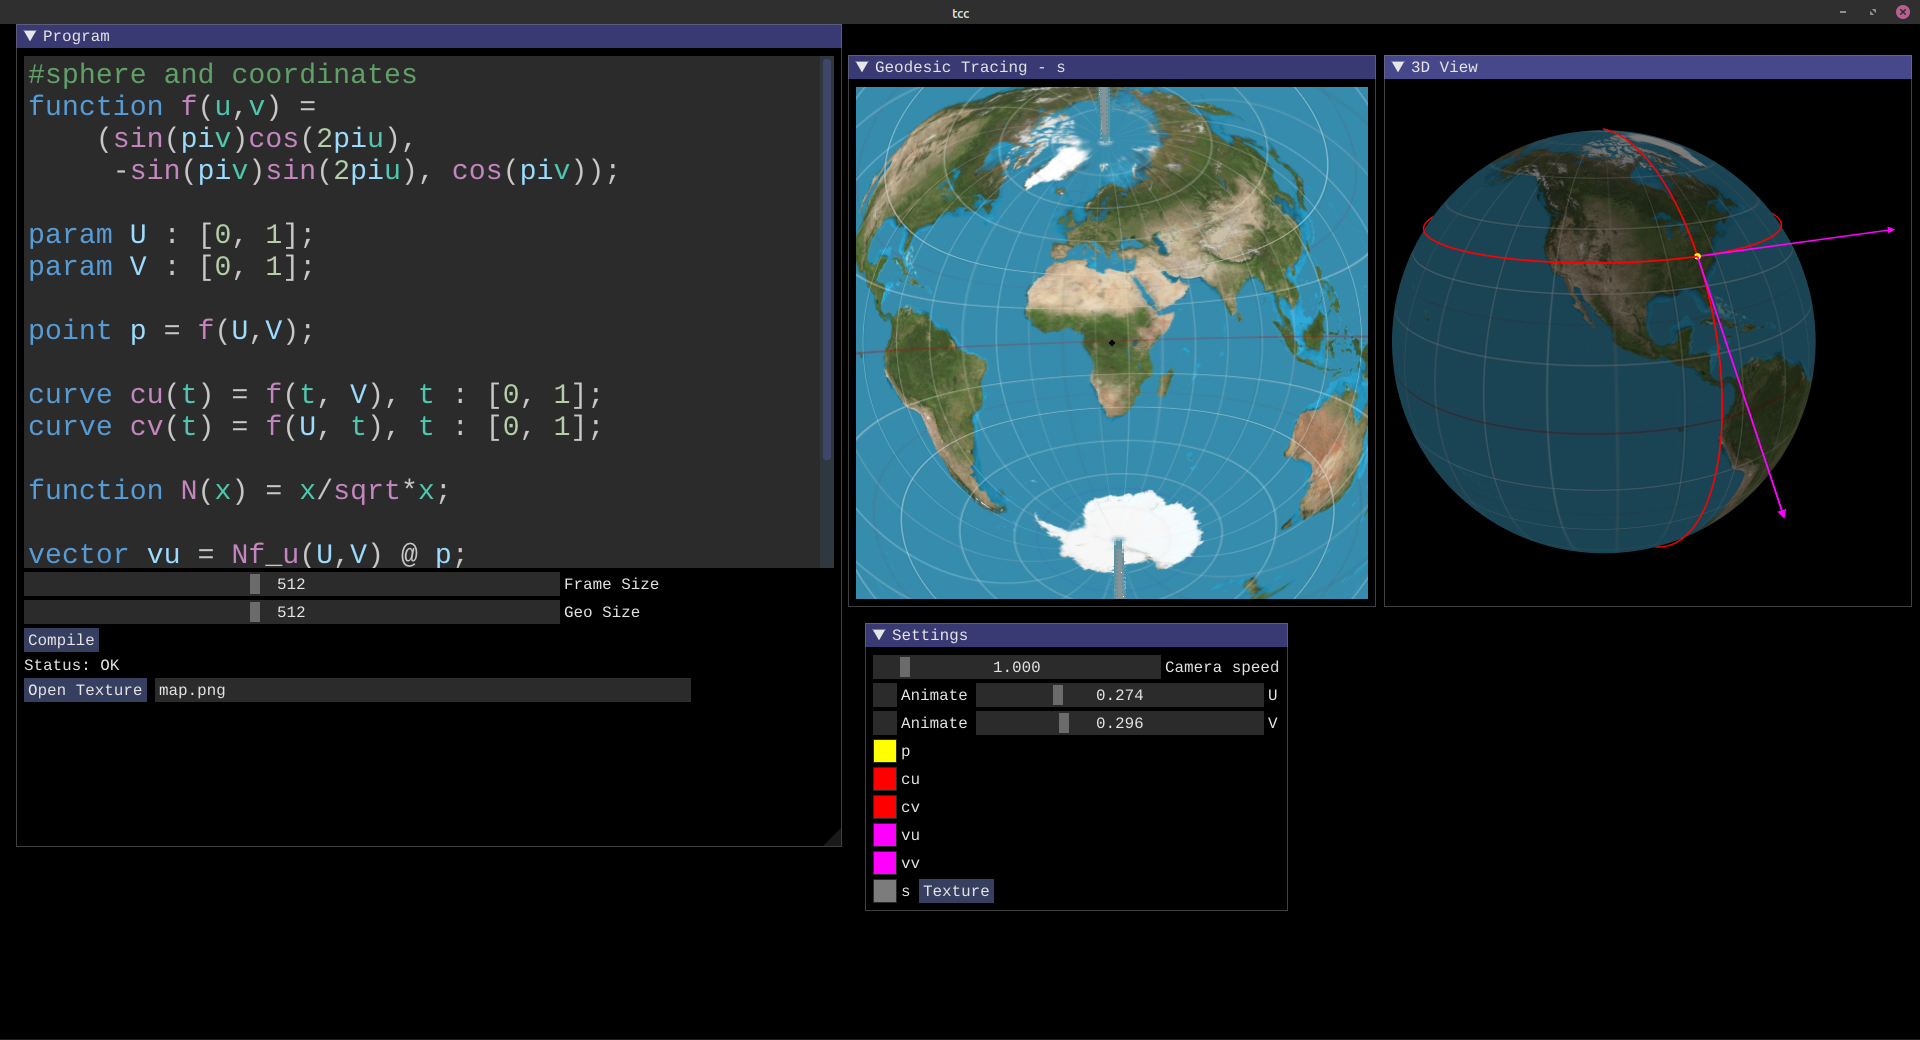
\includegraphics[width=\linewidth, frame]{preview.png}
    \caption{Exemplo da visualização}
    \label{img:preview}
\end{figure}

\newpage

A Figura \ref{img:chart} representa os estágios da aplicação.

\begin{figure}[!ht]
    \centering
    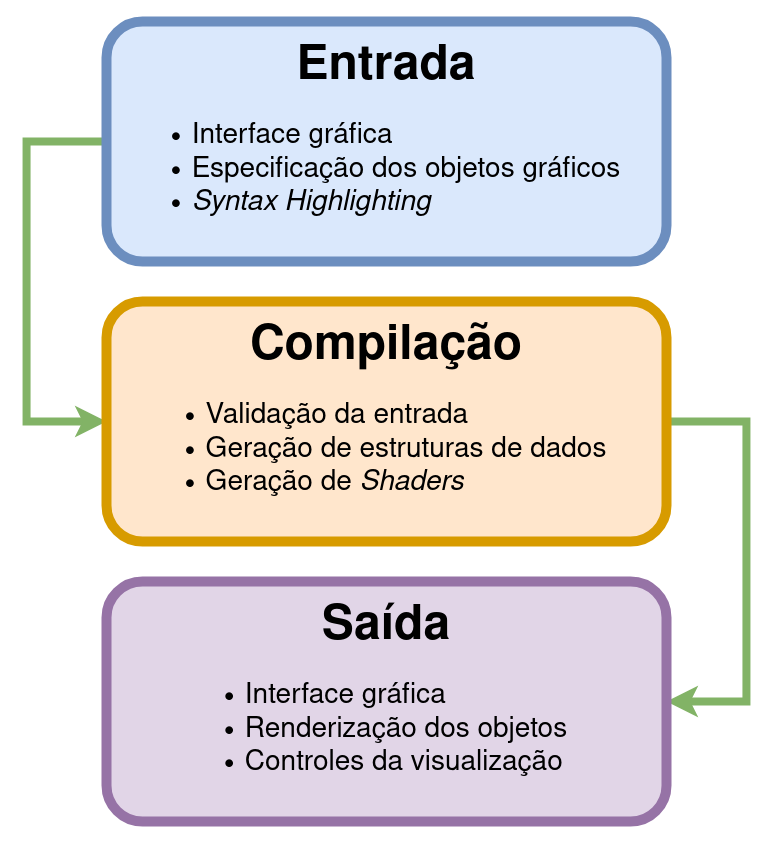
\includegraphics[width=0.6\linewidth]{chart.png}
    \caption{Estágios da aplicação}
    \label{img:chart}
\end{figure}

A entrada se refere ao texto que o usuário escreve para definir os objetos matemáticos.
O texto é digitado na própria interface gráfica, numa caixa de texto multilinha
e com \textit{Syntax Highlighting}: cores associadas às palavras e símbolos.

A compilação se refere ao processamento da entrada.
Eventualmente, o usuário pode cometer erros sintáticos ou semânticos.
Esses erros são detectados no compilador, e uma mensagem de erro é emitida.
Se o texto for válido, várias estruturas de dados são geradas,
com todas as informações relevantes sobre os objetos. Além disso,
\textit{Shaders} são gerados e compilados.
Cada \textit{shader} faz a renderização de um objeto.
Para superfícies, um outro \textit{shader} é necessário para fazer o \textit{Geodesic Tracing}.

A saída se refere ao produto final da compilação.
Todos os objetos são desenhados na interface gráfica.
Além disso, o usuário pode controlar vários aspectos da visualização,
como a câmera, e controles deslizantes para os parâmetros.

Todos os arquivos necessários para a compilação dessa aplicação se encontram
no repositório público \cite{TCC}. Todos os códigos são abertos e livres.